\documentclass[10pt,conference]{IEEEtran}
\IEEEoverridecommandlockouts
% ICSE 2027 Research Track -- IEEE conference template

%%%%%%%%%%%%%%%%%%%%%%%%%%%%%%%%%%%%%%%%%%%
%% PACKAGES
%%%%%%%%%%%%%%%%%%%%%%%%%%%%%%%%%%%%%%%%%%%
\usepackage{cite}
\usepackage[T1]{fontenc}
\usepackage[utf8]{inputenc}
\usepackage{amsmath,amssymb,amsfonts}
\usepackage{algorithmic}
\usepackage{algorithm}
\usepackage{graphicx}
\usepackage{textcomp}
\usepackage{xcolor}
\usepackage{multirow}
\usepackage{booktabs}
\usepackage{colortbl}
\usepackage{tcolorbox}
\usepackage{listings}
\usepackage{longtable}
\usepackage{array}
\usepackage{xspace}
\usepackage{siunitx}
\usepackage{balance}
\usepackage{adjustbox}
\usepackage[skip=2pt,font=footnotesize]{caption}
\usepackage{subcaption}
\usepackage{pgfplots}
\pgfplotsset{compat=1.18}
\usepgfplotslibrary{groupplots}
\usepackage{url}
\usepackage[hidelinks]{hyperref}
\usepackage[capitalise,nameinlink]{cleveref}
\usepackage[strict=true,english=american]{csquotes}
\usepackage{graphicx}
\usepackage{multirow}
\usepackage{environ}
\usepackage{tcolorbox}
\usepackage{soul}
\usepackage{listings}
\usepackage{balance}
% Character protrusion + font expansion: tightens line breaking (typically
% 1--2% shorter) without changing font size, margins, or wording. Improves,
% rather than degrades, readability. Used to help meet the 10-page text limit.
\usepackage{microtype}

%%%%%%%%%%%%%%%%%%%%%%%%%%%%%%%%%%%%%%%%%%%
%% COMMANDS
%%%%%%%%%%%%%%%%%%%%%%%%%%%%%%%%%%%%%%%%%%%
\newcommand\etal[0]{\emph{et al.}\xspace}
\newcommand{\ie}{\emph{i.e.,}\xspace}
\newcommand{\eg}{\emph{e.g.,}\xspace}
\newcommand{\cf}{\emph{cf.}}
\newcommand{\etc}{\emph{etc.}\xspace}
\newcommand{\wrt}{w.r.t.\xspace}
\newcommand\hoption[1]{\texttt{#1}}
\newcommand{\nbconfigurations}{1{,}152}
\newcommand{\percent}{\,\%}
%% ----------------------------------------------------------------------
%% Family and dataset macros
%% ----------------------------------------------------------------------
%% Family labels (the evidence families introduced in
%% Sec.~\ref{subsec:families}). Rendered in all caps as taxonomic
%% labels; \xspace handles trailing-space etiquette. Change once here
%% to restyle paper-wide.
\newcommand{\StudyReplication}{REPLICATION\xspace}
\newcommand{\StudyReplicationICSE}{REPLICATION-\allowbreak ICSE19\xspace}
\newcommand{\StudyReplicationICPE}{REPLICATION-\allowbreak ICPE20\xspace}
\newcommand{\StudyEnergy}{ENERGY\xspace}
\newcommand{\StudyWorkload}{WORKLOAD\xspace}
\newcommand{\StudyLCBench}{LCBENCH\xspace}
\newcommand{\StudyLinux}{LINUX\xspace}

%% Dataset/artifact names that are external publications worth citing
%% directly. Internal artifact names (the previous ``NewRuns'',
%% ``Twins'') are not used: families plus citations are clearer.
\newcommand{\dsXmat}{x264 ICPE\,2020}
\newcommand{\dsWLI}{workload-impact ICSE\,2023}
\newcommand{\dsLCBench}{LCBench\xspace}
\newcommand{\dsTux}{TuxKConfig}

\newcommand{\rqfinding}[2]{%
  \begin{tcolorbox}[
    colback=gray!6,
    colframe=black!60,
    title=\textbf{#1},
    fonttitle=\small,
    boxsep=0.7mm,
    left=2mm,right=2mm,top=1mm,bottom=1mm,
    before skip=3pt,after skip=3pt
  ]
  \small #2
  \end{tcolorbox}
}
\newcommand{\plusminus}{$\pm$\,}
\newcommand{\red}[1]{\textcolor{red}{#1}}

%% Notation conventions used throughout the paper
\newcommand{\TrainCost}{\mathit{TrainCost}}
\newcommand{\SizeCost}{\mathit{SizeCost}}
\newcommand{\FullCost}{\mathit{FullCost}}
\newcommand{\Ratio}{\mathit{Ratio}}
\newcommand{\Bias}{\mathit{Bias}}
\newcommand{\MRE}{\mathit{MRE}}

%% Column types reused from earlier draft
\newcolumntype{L}[1]{>{\raggedright\let\newline\\\arraybackslash\hspace{0pt}}m{#1}}
\newcolumntype{C}[1]{>{\centering\let\newline\\\arraybackslash\hspace{0pt}}m{#1}}
\newcolumntype{R}[1]{>{\raggedleft\let\newline\\\arraybackslash\hspace{0pt}}m{#1}}
\DeclareUnicodeCharacter{2212}{-}




%%%%%%%%%%%%%%%%%%%%%%%%%%%%%%%%%%%%%%%%%%%
%% Document
%%%%%%%%%%%%%%%%%%%%%%%%%%%%%%%%%%%%%%%%%%%
\begin{document}

\title{Sample Size Is Not Sampling Cost:\\A Construct-Validity Study of Performance\\ Prediction for Configurable Systems}
% Alternatives the authors considered (kept here as a record):
%   * "Sample Size or Sampling Cost? Performance Prediction of Configurable Systems Revisited"
%   * "From Sample Size to Sampling Cost in Performance Prediction of Configurable Systems"
%   * "Cost vs. Count in Sampling-Based Performance Prediction of Configurable Systems"

\author{\IEEEauthorblockN{Anonymous Author(s)}}

\maketitle

\begin{abstract}
Sampling-based performance prediction for configurable systems is usually
evaluated by accuracy and sample size. The assumption from several previous studies is that counting the number
of measured configurations is a valid proxy for acquisition cost. We test that
premise across six corpora: replications of Kaltenecker (ICSE'19) and Pereira
(ICPE'20, x264), performance--energy and workload-sensitive datasets, an
\StudyLCBench tuning corpus, and Linux kernel releases. We replace count-based
effort with measured cost, the sum of the measured costs of a strategy's training
sample, an acquisition cost except on Linux, where cost is image size and serves
as a resource-budget stress test.
Sample size is positively correlated with measured cost everywhere, so the proxy
is not arbitrary, but it is far from sufficient. Same-size samples can differ in
measured cost by more than an order of magnitude, and a larger sample can be
cheaper than a smaller one. Re-running the replication studies' own
Kruskal--Wallis sampler test at a fixed measured budget, rather than a fixed
sample size, changes the set of statistically tied-best samplers in $38$--$55\%$
of comparisons across the five non-Linux families and in all of them on Linux. Of
these, $12$--$55\%$ reproduce in $\ge95\%$ of bootstrap resamples, most robustly on
the replications and Linux. The measured-cost Pareto-efficient choice set robustly
differs from the count-based one in $73$--$100\%$ of scenarios, the more stable
decision-level evidence. Measuring cost also surfaces \emph{cost-aware}
samplers the count view cannot see, which reach better accuracy at the same
measured budget. For researchers and practitioners, the lesson is concrete:
sampling efficiency cannot be claimed from sample count, because the count-best
sampler is frequently not the cost-effective one once cost is charged. These
results do not invalidate fixed-sample accuracy comparisons, but efficiency claims
based on sample count require measured-cost calibration.
\end{abstract}

\section{Introduction}
\label{sec:introduction}

Configurable software systems expose tens to hundreds of options whose
combinations form configuration spaces far too large to measure exhaustively,
and because each configuration must be built and executed before its
performance is known, every measurement is costly~\cite{julianasurvey}.
Performance prediction is therefore usually framed as
a sampling problem: measure a small set of configurations, train a model, and
use it to predict the rest of the configuration space
\cite{guo2013ASE,sarkar2015,siegmund2015FSE,kaltenecker2019,julianasurvey,JVKSK:SEAMS17,jamshidi2018,dorn2026bayesian}.
Since no single notion of a ``good'' sample dominates, many sampling strategies
have been proposed, from uniform \texttt{random} sampling and $t$-wise or
coverage-oriented designs to distance-based, diversity-driven, and more recent
uncertainty- or cost-aware schemes, each betting on a different rationale for
which configurations are most informative to
measure~\cite{guo2013ASE,DBLP:journals/tse/HenardPPKHT14,kaltenecker2019,sarkar2015,nair2018c}.
% \hl{Different sample strategies pursue different objectives. \texttt{Random} selects configurations uniformly at random, \texttt{balanced} aims to improve coverage of option values, \texttt{diversity} intentionally spreads samples across distant regions of the configuration space, \texttt{pairwise} emphasizes coverage of pairwise feature interactions, and \texttt{pilotCost} is a simple cost-aware strategy that favors configurations estimated to be inexpensive to measure. Regardless of the strategy, the selected configurations are executed to obtain the target labels (\textit{e.g.}, runtime or energy consumption), which are then used to train the prediction model.}
 Because measurements are expensive, sampling studies compare strategies on
accuracy and ``effort''. In these studies, effort often means the
number of measured configurations. A strategy that measures $64$
configurations is treated as twice as expensive as one that measures $32$, and
two strategies that both measure $64$ configurations are treated as equally
expensive.

That convention is useful, but it is also a hypothesis. It assumes that each
configuration costs roughly the same to measure, or at least that sampling
strategies do not systematically choose more expensive or cheaper regions of
the configuration space. Configurable systems give us many reasons to doubt
that assumption. In a video encoder, compression options can multiply encoding
time. In an archiver, compression settings can change energy consumption by
orders of magnitude. In a compiler, optimization passes can turn a short
compilation into a long one. In such settings, sample size remains a count,
but it may no longer be a budget.

\begin{figure*}[t]
\centering
\begin{subfigure}[t]{0.40\textwidth}
\vspace{0pt}
\scriptsize
\raggedright
\textbf{Sampling principle.}
A strategy selects $n$ configurations from the option space. The measured
runtime of those configurations is the measured cost, and their energy
labels train the predictor.
\[
\mathcal{C}\xrightarrow[\text{strategy }s]{n=16}S_{s,n},
\qquad
\TrainCost=\sum_{c\in S_{s,n}}\mathrm{runtime}(c)
\]

\vspace{-0.35em}
\noindent\textbf{Excerpt of selected rows.}\par
\vspace{0.15em}
\setlength{\tabcolsep}{1.9pt}
\renewcommand{\arraystretch}{0.85}
\begin{tabular}{@{}l ccccc @{\hspace{5pt}} rr@{}}
\toprule
 & \multicolumn{5}{c}{\textbf{Options} {\tiny(what we choose)}}
 & \multicolumn{2}{c}{\textbf{Measured} {\tiny(what we pay / learn)}} \\
\cmidrule(lr){2-6}\cmidrule(l){7-8}
Strategy & enc. & comp. & method & lev. & cores & runtime & energy \\
 & & & & & & {\tiny cost (ms)} & {\tiny label (J)} \\
\midrule
pilotCost & off & off & none & $1$ & $1$ & $10.3$k & $421$ \\
pilotCost & off & off & none & $2$ & $3$ & $10.4$k & $423$ \\
pilotCost & on  & off & none & $7$ & $1$ & $13.7$k & $537$ \\
\midrule
diversity & on  & on & zpaq & $9$ & $1$ & $1.66$M & $53.6$k \\
diversity & off & on & zpaq & $9$ & $1$ & $1.61$M & $51.8$k \\
diversity & off & on & lzma & $9$ & $4$ & $288$k & $9.52$k \\
\bottomrule
\end{tabular}

\vspace{0.25em}
\caption{Three of each strategy's $16$ measured configurations. \texttt{pilotCost}
selects cheap-to-run ones, \texttt{diversity} expensive ones.}
\label{fig:re-table}
\end{subfigure}\hfill
\begin{subfigure}[t]{0.57\textwidth}
\vspace{0pt}
\centering
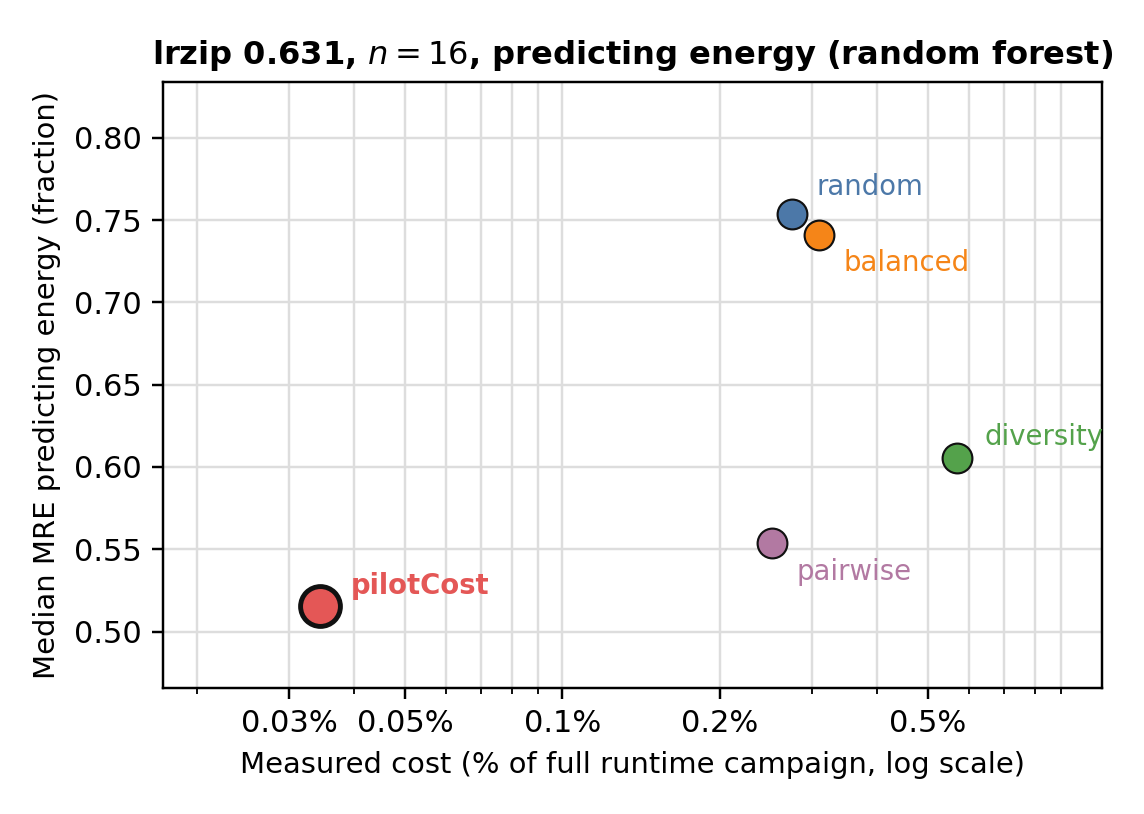
\includegraphics[width=0.75\linewidth]{pic/results/lrzip_fig1_rf_strictwin.png}
\caption{Same count, $>$order-of-magnitude measured-cost spread.}
\label{fig:re-scatter}
\end{subfigure}
\caption{Running example (lrzip 0.631, predicting energy under a measured-runtime
budget, random forest). (a) three of each strategy's $16$ measured
configurations: runtime (ms) is the per-point cost, energy (J) the label fit.
(b) sample count prices all five strategies alike, yet measured cost
separates them by more than an order of magnitude, and the cheapest
(\texttt{pilotCost}) is also the most accurate (learner-independent). Numbers in
text.}
\label{fig:running-example}
\end{figure*}

%The issue is not merely accounting. 
\Cref{fig:running-example} illustrates why treating sample size as a proxy for acquisition cost can be misleading. 
\Cref{fig:re-table} shows a subset of the sampled configurations ($n=3$ for \texttt{pilotCost} and \texttt{diversity}) on the lrzip subject from our performance-energy corpus.
%\Cref{fig:running-example} gives the smallest version of the phenomenon on a real subject: lrzip in the performance--energy corpus, where the goal is to predict energy but the budget is the measuredperformance cost of the training configurations (\Cref{fig:re-table}). 
\Cref{fig:re-scatter} summarizes the practical consequence ($n=3$ for five sampling strategies).
While all strategies measure the same $16$ configurations, so count-based effort assigns them
the same cost. Measured cost does not: \texttt{pilotCost}
spends only $0.03\%$ of the full budget while \texttt{diversity} spends $0.56\%$, a
$16.5\times$ gap counting cannot see, and \texttt{pilotCost} is also \emph{more
accurate} ($0.52$ vs.\ $0.61$ MRE, reported throughout as a fraction), strictly
dominating diversity on both axes. The reordering is not confined to the extremes:
\texttt{random} and \texttt{balanced} are cheaper than \texttt{diversity} yet less
accurate, a genuine cost--accuracy trade-off the count view hides. Sample size can
thus hide an order-of-magnitude cost difference, and even hide which strategy is
better, once cost is measured. Thus, our question is
not only whether $n$ correlates with cost in aggregate, but whether $n$ is a valid
cost axis for the sampling strategies a paper recommends, and whether the reversal
it shows is an isolated artifact of \Cref{fig:running-example} or a broader threat.

This paper's thesis is as follows: Sample size can order sampling effort, but treating it as the cost axis
is unsafe until the measured cost has been checked. In many
realistic scenarios, considering the actual cost changes the sampling strategy recommendation or the
set of efficient strategy--budget combinations.
This is not a blanket criticism of prior work. Sample size is practical,
reproducible, and often correlated with actual cost. Our claim is narrower:
when a paper makes a resource claim, the count proxy should be confronted against
the measured cost. A statement such as ``strategy $A$ is cheaper
than strategy $B$'' is only meaningful after specifying whether ``cheaper''
means fewer configurations or less measured cost.

We test the size-as-cost abstraction by replacing count-based effort with the
\emph{measured cost} of a strategy's training sample: the sum of the
per-configuration costs actually measured to acquire it, written $\TrainCost$.
This measured cost is the sampling cost our title sets against sample size. We
also call it an \emph{acquisition cost} when the point is what the resource is
spent on, namely the labels acquired for training, and otherwise use the shorter
\emph{measured cost} throughout. We study six families of experiments: (i) a
\StudyReplicationICSE revisit of Kaltenecker-style configurable-system
traces~\cite{kaltenecker2019}, (ii) a \StudyReplicationICPE revisit of x264~\cite{pereira2020}, %over $17$ inputs and two targets~\cite{pereira2020}, 
(iii) a performance--energy
corpus~\cite{weber2023twins}, (iv) a workload-impact corpus with $93$
system--workload contexts~\cite{muhlbauer2023workload}, (v) an \StudyLCBench
external-validation corpus with $35$ OpenML datasets and runtime learning
curves~\cite{zimmer2021autopytorch}, and (vi) six Linux kernel
releases~\cite{martin2022linux,borges2025linux}. We ask three research questions:
\emph{(1)}~to what extent sample size reflects measured cost,
\emph{(2)}~whether replacing sample size by measured cost changes
sampling-strategy conclusions, and \emph{(3)}~under which conditions sample size
is a safe or unsafe cost proxy. Agreement or disagreement across families is
itself part of the result.

The novelty is not the observation that configurations have heterogeneous
cost. %That much is expected. 
It is that the standard sample-count effort axis,
re-evaluated under measured cost, changes \emph{which samplers are
statistically recommendable} and \emph{which strategy--budget menus are
Pareto-efficient}, established with the original studies' own statistical test
rather than a new one of our choosing. Our contributions are as follows:

% \noindent\textbf{Contributions.}
\begin{itemize}
    \item We operationalize measured cost as an evaluation axis and
    define metrics that test
    when sample size can stand in for it.
    \item We quantify the decision impact by re-running the replication studies'
    own Kruskal--Wallis sampler test and Pareto choice-set analysis under measured
    cost, which change both the statistically recommendable samplers and the
    efficient strategy--budget menu.
    \item We show that measuring cost surfaces \emph{cost-aware} samplers that
    are off the radar under sample count, and give an existence proof:
    \texttt{pilotCost}, a deliberately simple pilot of cost-aware sampling, is on
    several systems the most cost-effective choice: better accuracy at equal sample size.
    %measured cost.
    \item We identify validity conditions and reporting guidance: count-based
    conclusions are most defensible on homogeneous, cost-unaware regimes, and
    fragile under heavy-tailed costs, target--cost asymmetry, workload/context
    shifts, and diversity or active-learning samplers.
\end{itemize}

\section{Background and Related Work}
\label{sec:background}
\label{sec:related_work}

A configurable system exposes options whose valid combinations form a configuration space $C$. For a fixed workload and non-functional property, each
configuration $c\in C$ has a measured value $y_c$ such as runtime, output size,
or energy. Sampling-based performance prediction trains a regression model
$\hat y$ from a measured subset $S\subset C$ and evaluates prediction error,
typically mean relative error
($\MRE=(1/|T|)\sum_{c\in T}|y_c-\hat y_c|/|y_c|$, lower is better), on
held-out configurations $T$~\cite{siegmund2015FSE,kaltenecker2019,pereira2020,julianasurvey}.

\paragraph*{Sampling strategies}
The configurable-systems literature offers several domain-agnostic families.
Random sampling draws configurations uniformly. Solver-based sampling asks
SAT/SMT solvers (Sat4j, Z3) for valid configurations, and its randomized variant
perturbs solver order for diversity \cite{DBLP:journals/tse/HenardPPKHT14}.
$t$-wise sampling covers option-value combinations
\cite{Kuhn2004,Cohen2008,Johansen2012}. Distance-based and diversified
distance-based sampling spread the sample in feature space \cite{kaltenecker2019}.
When artifacts provide measured pools rather than feature-model handles, we use
pool-based analogues: \emph{balanced} keeps option frequencies close to the pool,
\emph{coverage} matches marginal option coverage, \emph{diversity} spreads by
Hamming distance, \emph{uncertainty} adds high-residual configurations,
\emph{pairwise} covers option-value pairs, and \emph{pilot-cost} learns a small
pilot cost model before choosing configurations predicted inexpensive.

\paragraph*{How prior work counts effort.}
Sampling-based performance prediction has studied random, solver-based,
coverage-based, distance-based, progressive, and transfer-learning strategies
\cite{guo2013ASE,sarkar2015,siegmund2015FSE,nair2018c,kaltenecker2019,julianasurvey},
and almost all of them equate measurement effort with sample size. Sarkar
\etal, the closest cost-aware precedent, define a composite objective with
training, testing, model, and error cost, but collapse acquisition effort to a
term proportional to $n$ under unit per-configuration cost \cite{sarkar2015}.
Westermann \etal discuss the number of measurement points needed for a target
error \cite{westermann2012}. Guo \etal vary measurement budgets ($N$, $2N$,
$3N$, and a larger reference $M$) \cite{guo2013ASE}. Siegmund \etal report
Pareto trade-offs between accuracy and number of measurements
\cite{siegmund2015FSE}. Kaltenecker \etal compare strategies at common
sample sizes \cite{kaltenecker2019}. Siegmund \etal also report elapsed hours
for some heuristics \cite{siegmund2012a}, but not as a test of whether $n$ is a
valid cost proxy. To our knowledge the proxy itself has not been evaluated in
this literature: our contribution is not a new sampler but a validity study of
that effort axis.

% NOTE: merged into Section II "Background and Related Work" (\input'd right after
% 2-background.tex). The section header and the "Sampling configurable systems"
% paragraph were folded into the merged "How prior work counts effort" paragraph
% there. The remaining paragraphs continue Section II.
\paragraph*{Counting effort versus measuring acquisition cost.}
Beyond the configurable-systems predecessors revisited in \Cref{sec:background},
the same count-as-effort convention recurs across tuning, transfer, and
prediction: ``effort,'' ``efficiency,'' and ``speedup'' are often expressed as
counts, that is, measurements, evaluations, queries, or target-environment
samples, because counts are simple to compare and reuse
\cite{nair2020flash,chen2021mmo,chen2024admmo,ye2025dlisa,gong2023dal,gong2024sempl}.
Counts sound like budgets only if one count unit stands for a comparable amount
of acquisition cost. Otherwise, a cost-effective result can be an accuracy
result wearing a cost label. Even work explicitly framed around cost, such as
cost-efficient sampling \cite{sarkar2015}, still prices each configuration as one
unit, whereas we audit its \emph{measured} cost. This does not invalidate prior accuracy results: a
fixed-$n$ comparison answers a legitimate accuracy question, and only the added
efficiency or budget reading needs measured-cost calibration. Some tuning work
already grounds counts in measured wall-clock budgets
\cite{chen2021multiobj,chen2023aspirations}, while our results show why
per-configuration and per-strategy calibration is still needed.

\paragraph*{Surrogate and heterogeneous costs.}
Replacing a real resource with an easy-to-count surrogate is a recurring
validity concern. In mutation testing, for example, the number of mutants can
mislead relative to execution time \cite{harmanMutationFSE2020}. We ask the
analogous question for configuration sampling, but the mechanism and the
contribution differ from that precedent in three ways. First, the driver is
\emph{strategy bias}: sampling strategies systematically steer toward cheap or
costly regions, so equal-size samples from different strategies spend unequal
measured budgets. There is no analogue of a sampling strategy in mutant
counting. Second, the acquisition cost and the prediction target can be
\emph{different} measured quantities (predicting output size while paying
encoding time), an asymmetry with no mutation-testing counterpart. Third, we do
not merely flag the threat: we quantify its decision impact by re-running the
original studies' own Kruskal--Wallis test under measured cost, and we identify
the conditions (cost heterogeneity, strategy bias, and target--cost
asymmetry) under which the proxy breaks. The surface observation that
configurations have heterogeneous cost is not the contribution. The contribution
is that this changes the set of statistically recommendable samplers and the
efficient sets.

\paragraph*{Context, learners, and optimization.}
Prior work shows that sampling conclusions can vary across inputs, workloads,
and target properties \cite{pereira2020,ye2026domland}, and we use these dimensions
to test cost-proxy validity. Learner choice is a separate modeling issue: we
keep literature-aligned learners for replications and use stronger sklearn
baselines as robustness checks or primary learners for newly framed families
\cite{breiman2001random,valov2015,amand2019,bao2018,sklearn_api}. Active
learning and multi-objective optimization offer candidate solutions, but they
inherit the same proxy question through their cost term
\cite{sarkar2015,siegmund2015FSE,li2020pareto}. We therefore treat measured
cost as a prerequisite for accuracy--cost claims, not as a new optimizer. A
complementary strand instead measures model-building or adaptation cost rather
than label acquisition: training time \cite{gong2022encoding}, online-drift
overhead \cite{xiang2026dhda}, and deep-learning costs \cite{gong2024dcpl}.
Extending our audit to those axes is future work.
    % continues Section II (Background and Related Work)
\section{Cost Model}
\label{sec:cost_model}

For a run $r$ of strategy $s$ at training size $n$, let
$S_{r,s,n}\subseteq C$ be the selected sample. The usual cost model is the
count of measured configurations:
\begin{equation}
\SizeCost(s,n)=n.
\label{eq:sizecost}
\end{equation}
We compare it with the measured cost:
\begin{equation}
\TrainCost(r,s,n)=\sum_{c\in S_{r,s,n}}\mathit{cost}(c).
\label{eq:traincost}
\end{equation}
Here $\mathit{cost}(c)$ is the measured resource consumed for configuration $c$:
wall-clock measurement time in most of our study, energy in the
performance--energy family, and the uncompressed \texttt{vmlinux} size in the
Linux family. The first two are label-acquisition costs. Image size is instead a
resource budget (the shippable footprint that constrains embedded and
over-the-air deployment), so we rest the acquisition-cost claim on the five
families where cost is acquisition cost and treat Linux as a resource-budget
stress test that isolates strategy-induced selection bias alone: there the
prediction target and the paid resource coincide, leaving no target--cost
asymmetry to exploit (\Cref{subsec:results-rq3}). The model does not require the
cost dimension to equal the prediction target: one may predict output size while
paying time, or runtime while paying energy.

To compare systems with different absolute costs, we normalize by the cost of
measuring the whole available configuration space:
\begin{align}
\FullCost &= \sum_{c\in C}\mathit{cost}(c),\\
\mathit{TrainCostPct} &= \frac{\TrainCost}{\FullCost},&
\mathit{SizePct} &= \frac{n}{|C|}.
\label{eq:pct}
\end{align}
$\FullCost$ is a retrospective normalizer for cross-system reporting only: the
$\Ratio$ and percentage views use it, whereas the strategy rankings and Pareto
fronts compare raw measured $\TrainCost$. A deployable sampler therefore never
needs $\FullCost$ in advance.
The count proxy has good \emph{budget agreement} when the fraction of
configurations measured matches the fraction of measured cost spent. We also
call this \emph{cost-proxy calibration}: the sample-size proxy is calibrated
when a $10\%$ sample spends about $10\%$ of the measured budget. This is not
statistical calibration of a prediction model. It is only a check that the cost
proxy is on the same scale as the measured resource. We summarize it with a
budget ratio:
\begin{equation}
\Ratio(r,s,n)=
\frac{\mathit{TrainCostPct}(r,s,n)}{\mathit{SizePct}(s,n)}.
\label{eq:ratio}
\end{equation}
$\Ratio=1$ means that a $10\%$ sample consumes about $10\%$ of the full
measurement cost. $\Ratio>1$ means the strategy selected costlier-than-average
configurations, whereas $\Ratio<1$ means it selected cheaper-than-average ones. This is
a per-run ratio, so one-number summaries report the median ratio unless stated
otherwise. The practical question is whether a same-size sample takes more or
less of the real budget than the count suggests.

For decision-level comparisons, we use two standard views. First, we rank
strategy--budget combinations, where each combination is one sampling strategy
at one budget level, with a normalized objective
\begin{align}
J^{\text{size}}_{\lambda} &= \widetilde{\MRE}+\lambda\widetilde{\SizeCost},\\
J^{\text{meas}}_{\lambda} &= \widetilde{\MRE}+\lambda\widetilde{\TrainCost},
\end{align}
where the cost weight $\lambda\in\{0.1,0.25,0.5,1,2,4,10\}$ spans
accuracy-heavy to cost-heavy choices. Second, we compare Pareto fronts in the
MRE--cost plane: a combination is efficient if no other combination has both
lower error and lower cost. The main threat we test is whether the recommended
strategy or the efficient set changes when $\SizeCost$ is replaced by
$\TrainCost$.

Here $\widetilde{\MRE}$ and the tilded cost term are each min-max scaled to
$[0,1]$ within a context, so error and cost are comparable, and $\lambda$ trades
one against the other: small $\lambda$ is accuracy-heavy, large $\lambda$
cost-heavy. We explore a range of $\lambda$, since no single accuracy-versus-cost
weight fits every setting.

This formulation clarifies how the conventional fixed-$n$ protocol fits our
analysis: when strategies are compared at the same sample size with sample count
as the cost axis, the cost term is constant and the ranking collapses to
MRE: the standard pure-accuracy reading, valid for that question. The extra
assumption appears when that fixed-$n$ comparison is read as a fixed-\emph{budget}
one. A resulting ``flip'' is then either a genuine trade-off (the count winner is
more accurate but more expensive under measured cost) or a \emph{domination} (a
different combination is no less accurate and no more expensive). Pareto fronts
expose the second case without choosing a $\lambda$: when the measured-cost front
contains combinations missing from the count-cost front, a size-only analysis has
hidden choices a practitioner might legitimately prefer.

We count only training acquisition. Validation measurements are part of the
experimental protocol and are the same across strategies. A sampling strategy
controls which training configurations is measured.

\section{Research Questions and Study Design}
\label{sec:study_design}
\label{sec:experiment}

The study asks one question: when is sample size a good enough proxy for
measured cost, and when does that shortcut change the substantive
conclusion? We organize the evaluation around three research questions.

%\begin{itemize}
    %\item 
    \textbf{RQ1. To what extent does sample size reflect measured
    acquisition cost?} We test whether same-size samples spend comparable
    measured budgets, whether larger samples reliably cost more, and whether a
    fixed fraction of configurations corresponds to the same fraction of
    measured cost.
    
    % \item 
    \textbf{RQ2. Does replacing sample size by measured cost
    change sampling-strategy conclusions?} We compare the top accuracy--cost
    choices and the Pareto-efficient choice sets under count-based cost and
    measured cost.
    
    % \item 
    \textbf{RQ3. Under which conditions is sample size a safe or unsafe
    cost proxy?} We analyze how the answer depends on cost heterogeneity,
    strategy bias, target--cost asymmetry, workload/input, release, and dataset
    family.
% \end{itemize}

\paragraph*{Operational tests.}
RQ1 first checks \emph{cost heterogeneity}. We use the coefficient of variation
(CV), the standard deviation divided by the mean, because it is unit-free: a
CV of $0.20$ means the standard deviation is $20\%$ of the mean whether the
resource is seconds, joules, or bytes, while a CV near $1$ means the spread is as
large as the average cost. CV is sensitive to broad dispersion, so we pair it
with $p_{90}/p_{10}$, the ratio between the $90$th and $10$th percentile costs.
This second statistic is robust and readable: $p_{90}/p_{10}=1.5$ means a
costly but non-extreme configuration costs $50\%$ more than a cheap but
non-extreme one, while a value near $47$ means the upper tail is about $47\times$
costlier. Fixed-$n$ strategy-effect tests then ask the operational question:
when two strategies both choose, say, $64$ configurations, do they nevertheless
visit systematically cheaper or costlier regions?

RQ1 also checks \emph{budget calibration}. Spearman $\rho$ between $n$ and
$\TrainCost$ asks only whether larger samples tend to cost more. The ratio
$\Ratio$ from \Cref{eq:ratio} asks the stricter budget question. If a system has
$1{,}000$ configurations and a sample measures $100$, then $\mathit{SizePct}=0.10$.
If those $100$ configurations spend $8\%$ of the full measured campaign, then
$\Ratio=0.08/0.10=0.8$: the sample is cheaper than its count suggests. If it
spends $15\%$, then $\Ratio=1.5$: the sample is costlier than its count
suggests.

RQ2 compares sampling conclusions under count and measured cost through three
complementary lenses, in decreasing order of how much they drive our claims.
\emph{(i)~Cost-controlled sampler comparison (primary).} The replication studies
we revisit pick the best sampler with a Kruskal--Wallis (KW) omnibus over each
sampler's per-seed error distribution and a Dunn post-hoc (Holm-adjusted, as in
the source studies) that reports the \emph{top group} of samplers not
significantly worse than the best
\cite{kruskal1952,kaltenecker2019,pereira2020}. We rerun that exact test and
change one thing: we hold the measured cost fixed instead of the
sample size. For each context we form a budget grid from the measured costs of
the predefined sample sizes. At a budget $b$ every sampler enters at the
\emph{largest predefined sample size whose median measured cost is at most~$b$},
the most data it can afford. This operating point is chosen without consulting
error, so no point is selected by test accuracy. We use it as a retrospective,
cost-indexed evaluation device, relying on observed or pilot-estimated sampler
costs rather than on test error. A sampler with no affordable size at~$b$ is excluded from
that comparison. We report whether the KW top group (the set of statistically
recommendable samplers) changes between the size- and cost-controlled views, and
how often the source study's own recommended sampler is \emph{evicted} from it.
Selecting instead the cheapest-error affordable size (a retrospective upper
envelope applied symmetrically to all samplers) leaves the conclusion unchanged
and is reported as a sensitivity check.
\emph{(ii)~Pareto choice set.} A combination is efficient if no other has both
lower error and lower measured cost. We test whether the measured-cost efficient
set differs from the count-cost one (Jaccard $<1$) and, since a single
observation could be noise, whether that difference reproduces under a
test-set-and-run bootstrap ($p_{\text{differ}}\ge0.95$). \emph{(iii)~Top-$1$
flip.} The single best strategy--budget combination under the objective $J$ may
change between count and measured cost. Because this lens considers only the
top-ranked combination, it is sensitive to small margins between near-tied
combinations, so we report it with a bootstrap robustness check and treat it as
secondary evidence. RQ3 interprets the same
statistics across contexts. We report $p$-values where they are meaningful, but
always pair them with practical thresholds: CV$\ge0.20$ or
$p_{90}/p_{10}\ge1.5$ for visible cost spread,
$|\widetilde{\Ratio}-1|\ge0.05$ for budget mismatch, and Jaccard $<1$ for a
changed efficient choice set. These thresholds are a-priori reporting
conventions fixed before analysis rather than tuned cutoffs. They only flag
where a difference is large enough to be worth reporting, and no conclusion
depends on the exact value. Full per-scope tests, $p$-values, and effect
sizes are in the supplementary artifact.

\subsection{Evidence Families}
\label{subsec:families}

We keep six evidence families separate because they stress different validity
conditions. Pooling them would give a larger number but a weaker explanation of
when the sample-size proxy is reliable. The two replication families keep the
link with published configurable-system sampling studies: one revisits seven
Kaltenecker-style systems, and the other revisits x264 over $17$ inputs and two
measured properties. The four extension families then change one condition at a
time: the cost dimension (performance versus energy), the workload or input, an
external hyperparameter-optimization corpus, and a large Linux storage-cost
setting.

The \StudyReplicationICSE family is the most conservative test. It reuses the
published strategy panel on seven Kaltenecker \etal\ systems
\cite{kaltenecker2019} ($432$--$68{,}640$ valid configurations and $11$--$54$
options each, one performance-like target also charged as cost): random,
solver-based, randomized solver-based, $t$-wise, distance-based, and diversified
distance-based sampling. It changes only the cost axis from sample count to
measured performance cost. If a count-based conclusion changes there, the change
is not caused by inventing a new sampler or a new benchmark. The
\StudyReplicationICPE family uses the same logic on x264 \cite{pereira2020}, but
adds context: the same $1{,}152$ configurations ($16$ binary options) are
observed on $17$ videos and two properties (encoding time and output size, in
four cost--target scenarios), so we can ask whether the cost proxy is safer when
target and acquisition cost are the same than when they differ.

The extension families deliberately broaden the construct, and the first two
reuse published ICSE 2023 measurement datasets rather than a sampling protocol.
We draw our own samples on their measured configurations, so any cost effect is a
property of the data and not of a re-run. \StudyEnergy asks whether the issue is
only about runtime or also appears when performance and energy can each be target
or cost (the Twins-or-False-Friends corpus \cite{weber2023twins}, fourteen systems,
$180$--$86{,}058$ configurations each, four scenarios per system). \StudyWorkload
keeps systems fixed but changes workloads, testing whether a cost-proxy conclusion
is a property of the system or of the system--workload pair (the M\"uhlbauer
\etal\ corpus \cite{muhlbauer2023workload}, nine systems, $191$--$6{,}764$
configurations, $93$ system--workload contexts, $25{,}258$ measurements, with cost
measured as wall time, or oriented throughput for H2). \StudyLCBench moves outside
configurable-software performance tables, drawing on the LCBench learning-curve
benchmark \cite{zimmer2021autopytorch}, and checks whether real runtime learning
curves in hyperparameter optimization show the same count-versus-cost gap ($35$
OpenML datasets, $2{,}000$ configurations and $7$ hyperparameters each, accuracy
as target and runtime as cost). \StudyLinux stresses scale and strategy behavior
on the TuxKConfig kernel-size datasets \cite{martin2022linux,borges2025linux}:
random, balanced, coverage, uncertainty, and diversity sample from large
randconfig pools ($19{,}952$--$92{,}562$ configurations, $494$--$497$ options
across six releases v4.15--v5.08), and the cost is the uncompressed
\texttt{vmlinux} image size, a resource-budget proxy rather than measurement time.
\subsection{Protocol}
\label{subsec:protocol}

For each available tuple of system, workload/input, target, strategy, training
size, and run, we replay or generate the training sample, compute
$\TrainCost$, train the predictor on configuration options only, and evaluate
MRE on held-out configurations. Stochastic strategies are repeated over
seeds, about $100$ runs per cell for the replication archives and $30$ for the
generated families. We exclude measured performance, energy, size, and runtime
columns from the feature matrix to avoid label leakage, especially when the
target and acquisition cost are different measured quantities.

\paragraph*{Strategy panels and diagnostic bounds.}
For the two replication families we reuse the published strategy panels and their
measured sampling traces directly: the same strategies and the same measured
configurations as Kaltenecker \etal\ \cite{kaltenecker2019} and Pereira \etal\
\cite{pereira2020}, changing only the cost axis. The generated families also add \texttt{pilotCost}, a deliberately simple
cost-aware sampler, as an existence proof rather than a tuned method. It measures
a random pilot ($20\%$ of the target size, at least four configurations, whose cost
is charged in $\TrainCost$), fits a ridge model of log cost on the configuration
options, and predicts every other configuration's cost. It then fills the sample
from the configurations predicted cheapest, by diversity sampling, so the result
stays inexpensive while spreading across the option space. Because the pilot is
charged and it uses no cost information the other samplers lack, its advantage is
a fair one. Two diagnostic bounds, \texttt{cheapOracle} and \texttt{expensiveOracle},
instead look at the true costs to pick the cheapest and the most expensive
configurations, bracketing what perfect cost-awareness could achieve. They are not
deployable and are never reported as recommendations.

\section{Results}
\label{sec:results}

\begin{table*}[t]
\centering
\caption{RQ1 cost structure and the RQ3 validity regime, by family. Sample size
\emph{orders} cost in every family (Spearman $\rho>0.7$, with
\StudyReplicationICSE\ $0.879$--$0.943$, \StudyEnergy\ $0.710$--$0.996$,
\StudyLinux\ near-monotone), so the table reports where it nonetheless fails
as a \emph{budget}. $\Ratio$ is the median train-cost share divided by the count
share $n/|C|$ ($\Ratio{=}1$ is calibrated), and ``cost spread'' is per-configuration
heterogeneity ($p_{90}/p_{10}$ or CV). Regime: \emph{validated} (count
conclusions survive), \emph{warning} (the efficient set changes but few top
choices flip), \emph{changed} (the recommendation itself moves). %RQ2 change \emph{magnitudes} are in \Cref{tab:rq-metrics}.
}
\label{tab:decision-summary}
\footnotesize
\setlength{\tabcolsep}{4pt}
\renewcommand{\arraystretch}{1}
\begin{tabular}{p{0.12\linewidth} p{0.13\linewidth} p{0.22\linewidth} p{0.40\linewidth}}
\toprule
Family & Budget $\Ratio$ & Cost spread & Validity regime \& main lesson \\
\midrule
\StudyReplicationICSE & $0.80$--${\sim}1$ & $p_{90}/p_{10}=1.2$ (LLVM)--$47$ (lrzip, BerkeleyDBC) & Validated (LLVM, Polly, Dune, HIPAcc) to warning (7z, BerkeleyDBC). Published claims can flip. \\
\StudyReplicationICPE & ${\approx}1$ (aggregate) & strategy-biased: Henard $<$ $t$-wise & Changed under time-cost/size-target asymmetry. \\
\StudyEnergy & $0.17$--${\sim}1$ & $p_{90}/p_{10}=1.2$--$149$, CV $\le7.1$ (jump3r) & Spans tight/validated (PostgreSQL, LLVM) to heavy-tailed/changed (brotli, kanzi). Validity is per-system. \\
\StudyWorkload & $0.66$--$1.06$ & varies by workload & Changed in most contexts. The workload sets cost validity. \\
\StudyLCBench & $0.67$--$1.01$ & CV $0.60$--$2.25$ & Changed. The gap is not confined to configurable software. \\
\StudyLinux & $1.0$ (random)--$1.5$ (diversity) & CV $0.99$--$1.43$ & Changed every release. Scale and image-size cost expose strategy bias. \\
\bottomrule
\end{tabular}
\end{table*}

\subsection{RQ1: Sample Size Orders Cost, But Does Not Budget It}
\label{subsec:results-rq1}

\begin{figure}[t]
\centering
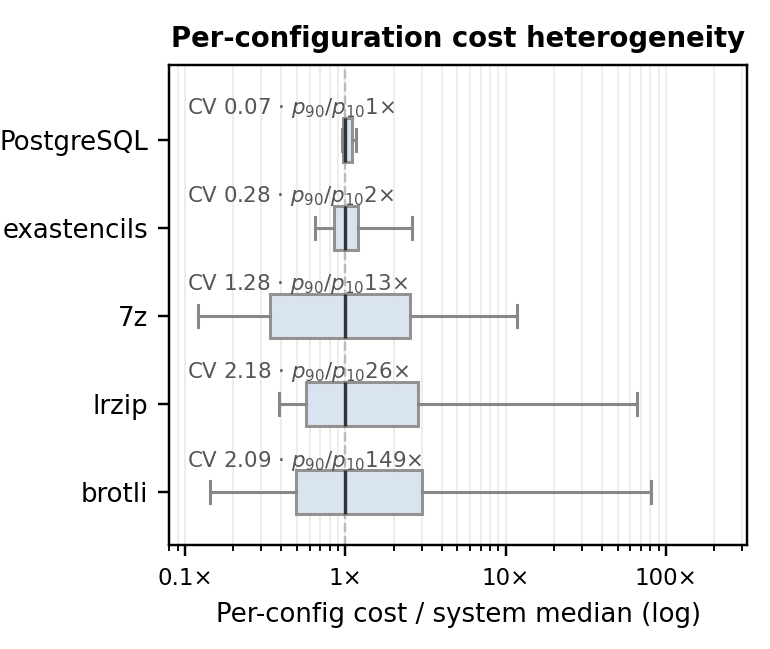
\includegraphics[width=0.88\columnwidth]{pic/results/fig_cost_distribution_regimes.png}
\caption{Per-configuration cost heterogeneity across energy systems: each box is
the per-config cost normalized by the system median (IQR box, min/max whiskers,
log scale), annotated with CV and $p_{90}/p_{10}$.}
\label{fig:distribution-regimes}
\end{figure}

\Cref{fig:distribution-regimes} illustrates the mechanism behind RQ1: how
strongly per-configuration costs vary within a system (CV and $p_{90}/p_{10}$
quantify the same spread). PostgreSQL is the validated extreme: costs are tight,
so sample count is a faithful budget proxy. As the distribution widens (7z,
lrzip, brotli) a fixed $n$ can spend wildly different measured budgets depending
on which configurations a strategy selects, which is what lets measured cost
re-order the sampler comparison.

Sample size is a useful ordering signal. In every family where we can test it,
larger samples are positively rank-correlated with measured cost.
This matters: count-based plots are not arbitrary, and $n$ remains a useful
common language for comparing sampling campaigns. In the
\StudyReplicationICSE revisit, Spearman correlation between sample size and
measured cost is high ($\rho=0.879$--$0.943$). The same ordering signal appears
in other families as well: \StudyEnergy remains positive even in its
hardest cases ($\rho=0.710$--$0.996$), and \StudyLinux is near monotone across
the six releases.

The failure is budget calibration. At fixed $n$, strategies can visit very
different cost regions: in the running example, five lrzip strategies all use
$n=16$ yet span a $16.5\times$ measured-cost gap for nearly identical MRE
(\Cref{fig:running-example}). Across families the cost spread ranges from benign
(LLVM $p_{90}/p_{10}=1.21$) to heavy-tailed (brotli $p_{90}/p_{10}=149$, lrzip and
BerkeleyDBC $\approx47$, jump3r CV $7.1$, Linux CV up to $1.4$,
\StudyLCBench CV up to $2.25$), with the \StudyEnergy family alone spanning both
extremes, and the
budget ratio drifts from calibrated to far below one (\StudyEnergy reaches
$\Ratio=0.17$, BerkeleyDBC $0.80$, workload and \StudyLCBench spanning
$0.66$--$1.06$).

This spread is strong enough to invert the size ordering itself. Within a single
strategy a larger sample almost never costs less ($<1\%$ of size pairs: cost is
monotone in a strategy's own $n$). \emph{Across} strategies it is common: a larger
sample drawn by a cheap sampler routinely undercuts a smaller sample drawn by a
costlier one. This cross-strategy reversal occurs in $11\%$ of \StudyEnergy\
comparisons and at least once in $79\%$ of its contexts, yet under the homogeneous
costs of the replication archives it is essentially absent ($\le 0.8\%$). The
count axis can thus not only mis-scale the budget but reverse it, and only where
costs are heavy-tailed, that is, where a few configurations are far more expensive
than the rest, the unsafe regime we analyze in \Cref{subsec:results-rq3}.

The x264 revisit explains why aggregate calibration is not enough. Its time
budgets look well calibrated when averaged over inputs, yet strategies are not
interchangeable: Henard-style samples tend to be cheaper, whereas $t$-wise
samples tend to be costlier. Thus a family can pass the coarse ``does $n$ order
cost?'' check and still fail the same-size, strategy-specific budget check that
matters for recommendations.


These three checks can disagree, and strategy bias, whether two same-$n$ samples
spend different budgets, is the mechanism behind most practical failures. On
Linux, random-like strategies stay close to the count budget while diversity costs
$1.24$--$1.52\times$ its count share, so an aggregate plot can look safe while a
specific strategy is not. \Cref{fig:running-example} is the sharpest local
instance: five strategies tied at $n{=}16$ yet separated by $16.5\times$ in
measured cost.

\rqfinding{Answer to RQ1}{Sample size is a useful ordering variable, but it is
not a calibrated budget. Across all families, larger samples usually cost more.
Nevertheless, same-size samples can differ by orders of magnitude in measured
cost, and across strategies a larger sample of a cheap sampler can be cheaper than
a smaller one of a costlier sampler ($11\%$ of \StudyEnergy\ comparisons), though
this is near-absent under homogeneous costs.}

\subsection{RQ2: Measured Cost Changes Strategy Assessment}
\label{subsec:results-rq2}

We read RQ2 through the three lenses of \Cref{sec:study_design}: the
cost-controlled Kruskal--Wallis (KW) sampler comparison (primary), the Pareto
choice set (robust, decision-level), and the top-$1$ flip (a narrow
illustration). The headline is the KW result. Each sampler enters at the largest predefined
sample affordable at a common measured budget (\Cref{sec:study_design}), and the
retrospective cheapest-error envelope, reported as a sensitivity check, agrees. Rerunning the replication studies' own
best-sampler test this way, instead of at a fixed sample size, the top group of
statistically
recommendable samplers changes in $8/21$ \StudyReplicationICSE comparisons
($38\%$), $28/51$ x264 comparisons ($55\%$), $56/112$ \StudyEnergy comparisons
($50\%$), $389/846$ \StudyWorkload contexts ($46\%$), and (outside configurable
software) $146/350$ \StudyLCBench datasets ($42\%$): $38$--$55\%$ across the five
non-Linux families. \StudyLinux is the extreme case rather than the exception:
even though its target \emph{is} the acquisition cost (\texttt{vmlinux} size),
strategy-level cost bias reshuffles the top group in all $30$ corrected
comparisons ($100\%$).

To check that these changes are not single-draw artifacts, we bootstrap the
membership change itself: resample each sampler's per-seed errors, recompute both
Dunn top groups ($B{=}1000$), and ask how often the change reproduces. It is
highly reproducible on the families that ground the published-verdict claim (all
x264 changes, $93\%$ on \StudyLinux, and $75\%$ on \StudyReplicationICSE), bbut
only a third to a half of the changes ($29$--$52\%$) reproduce on
\StudyEnergy/\StudyWorkload/\StudyLCBench, where the tied-best samplers are
near-ties (equal-budget MRE gaps of $0.2$--$2.0$pp). The recommendation-level
signal is sharper: the source study's own recommended sampler is \emph{evicted}
from the cost-controlled top group in $29$--$41\%$ of replication comparisons.
The omnibus KW remains significant in both views in $74$--$100\%$ of comparisons.
\Cref{tab:rq-metrics} collects the per-family numbers for both robust lenses.

\begin{table*}[t]
\centering
\caption{RQ2 across families: how often measured cost changes the conclusion
relative to sample count. \textbf{Kruskal--Wallis (KW)} reruns each study's own
best-sampler test at a fixed measured budget versus a fixed sample size.
\emph{Top-group~$\Delta$} is how often the Dunn/Holm set of statistically
tied-best samplers changes. \emph{Robust~$\Delta$} is the subset that reproduces in
$\ge95\%$ of seed-bootstrap resamples ($B{=}1000$). \emph{Evicted} is how often the
source study's own recommended sampler drops out of the cost-controlled top
group. \textbf{Pareto} gives how often the measured-cost efficient choice set
differs from the count one, reproducibly under the bootstrap
($p_{\text{differ}}\ge0.95$). \emph{Med.\ Jaccard} is the effect size (lower $=$
menus share fewer designs). The omnibus KW is significant in \emph{both} views in
$74$--$100\%$ of comparisons, and equal-budget MRE gaps on changed comparisons
are small ($0.2$--$3.9$pp). Comparison counts $N$ (KW/Pareto):
\StudyReplicationICSE\ $21/7$, x264 $51/17$, \StudyEnergy\ $112/56$,
\StudyWorkload\ $846/93$, \StudyLCBench\ $350/35$, \StudyLinux\ $30/6$. The
broader top-$1$ decision flip across cost weights ($32\%$, $538/1{,}666$, discussed
below) is a separate, weaker lens.}
\label{tab:rq-metrics}
\small
\setlength{\tabcolsep}{6pt}
\renewcommand{\arraystretch}{1.05}
\begin{tabular}{l ccc cc}
\toprule
& \multicolumn{3}{c}{Kruskal--Wallis sampler test} & \multicolumn{2}{c}{Pareto choice set} \\
\cmidrule(lr){2-4}\cmidrule(lr){5-6}
Family & top-group $\Delta$ & robust $\Delta$ & evicted & differs & med.\ Jaccard \\
\midrule
\StudyReplicationICSE\ (Kaltenecker~\cite{kaltenecker2019}, 7 systems) & $38\%$  & $29\%$ & $29\%$ & $86\%$  & $0.50$ \\
\StudyReplicationICPE\ (x264~\cite{pereira2020}, 17 inputs) & $55\%$  & $55\%$ & $41\%$ & $100\%$ & $0.33$ \\
\StudyEnergy\ (ICSE'23~\cite{weber2023twins}, 14 systems) & $50\%$  & $26\%$ & $17\%$ & $80\%$  & $0.65$ \\
\StudyWorkload\ (ICSE'23~\cite{muhlbauer2023workload}, 9 systems, 93 contexts) & $46\%$  & $21\%$ & $14\%$ & $73\%$  & $0.60$ \\
\StudyLCBench\ (LCBench~\cite{zimmer2021autopytorch}, 35 datasets) & $42\%$  & $12\%$ & $11\%$ & $89\%$  & $0.62$ \\
\StudyLinux\ (TuxKConfig~\cite{martin2022linux}, 6 releases) & $100\%$ & $93\%$ & $23\%$ & $100\%$ & $0.38$ \\
\midrule
Range                                & $38$--$100\%$ & $12$--$93\%$ & $11$--$41\%$ & $73$--$100\%$ & $0.33$--$0.65$ \\
\bottomrule
\end{tabular}
\end{table*}

This is a direct revisit of the replication studies' conclusions. Before
changing the cost axis we confirmed that our size-controlled replay reproduces
the source studies' fixed-$n$ verdicts: the size-view KW top groups
qualitatively match their reported outcomes (random a strong baseline across most
\StudyReplicationICSE systems, solver-based and $t$-wise competitive on x264), so
the changes reported below are attributable to the measured-cost axis rather than
a divergent replication. Kaltenecker
\etal\ \cite{kaltenecker2019} find distance-based samplers competitive at a fixed
sample size. At a fixed measured cost, diversified distance-based sampling falls
from best in $4$ comparisons to $1$, plain distance-based rises from $0$ to $2$,
and random stays dominant ($11$): \eg LLVM at the largest budget moves
\texttt{divDistBased}$\to$\texttt{random}, Polly
\texttt{solverBased}$\to$\texttt{random}. Pereira \etal\ \cite{pereira2020} show
x264 rankings shifting across inputs and targets. We add an orthogonal axis,
holding input and target fixed and changing only count\,$\to$\,measured cost:
\texttt{solverBased}, which selects expensive configurations, drops from best in
$12$ comparisons to $5$, while \texttt{divDistBased} rises from $7$ to $14$ (\eg
x264 input~$4$ at $t_1$ moves \texttt{solverBased}$\to$\texttt{divDistBased}). The
direction is consistent and mechanistic: at an equal budget an expensive sampler
cannot afford as large a sample, so it loses to cheaper samplers that buy more
data (see \Cref{subsec:results-rq3}). %\Cref{subsec:results-rq3} returns to why.

The choice-set lens is broader and the most robust. The measured-cost
Pareto-efficient set of strategy--budget combinations differs from the count-cost
set in almost every scenario, and the difference reproduces under the bootstrap
($p_{\text{differ}}\ge0.95$): in $45/56$ \StudyEnergy scenarios ($80\%$),
$68/93$ \StudyWorkload contexts ($73\%$), $31/35$ \StudyLCBench datasets
($89\%$), all $17$ x264 scenarios, and $6/7$ \StudyReplicationICSE systems, with
median Jaccard $0.60$--$0.65$. Even when the single best buy is stable, the menu
of efficient options a practitioner would compare is almost always different, and
that difference is not an artifact of one resampling. \Cref{fig:choiceset}
makes this concrete on the running example. On lrzip the count view's efficient
menu and the measured-cost menu share only $7$ of the $19$ designs either
certifies (Jaccard $0.37$): measured cost \emph{adds} $11$ designs the count view
discarded as ``too many samples'' (mostly large-$n$ \texttt{pilotCost} runs that
are cheap to measure) and drops $1$ it had kept. The efficient menu a
practitioner would compare is therefore not a refinement of the count one but a
genuinely different set. \StudyLinux, far from
being an exception, is the most extreme case. One might expect it to be safe: its
target \emph{is} the cost (\texttt{vmlinux} size), so $n$ tracks cost in
aggregate, yet with a full-feature learner the top group changes in all $30$
comparisons ($100\%$) and the choice set robustly differs on every release
($6/6$, median Jaccard $0.38$). The reason is exactly RQ1: even when count and
cost agree on average, strategy bias (diversity costs
$1.24$--$1.52\times$ its count share, active learning drifts) makes same-size
samples spend very different budgets, so the cost-controlled ranking still moves.
\Cref{tab:decision-summary} locates these changes by family.

\begin{figure}[t]
\centering
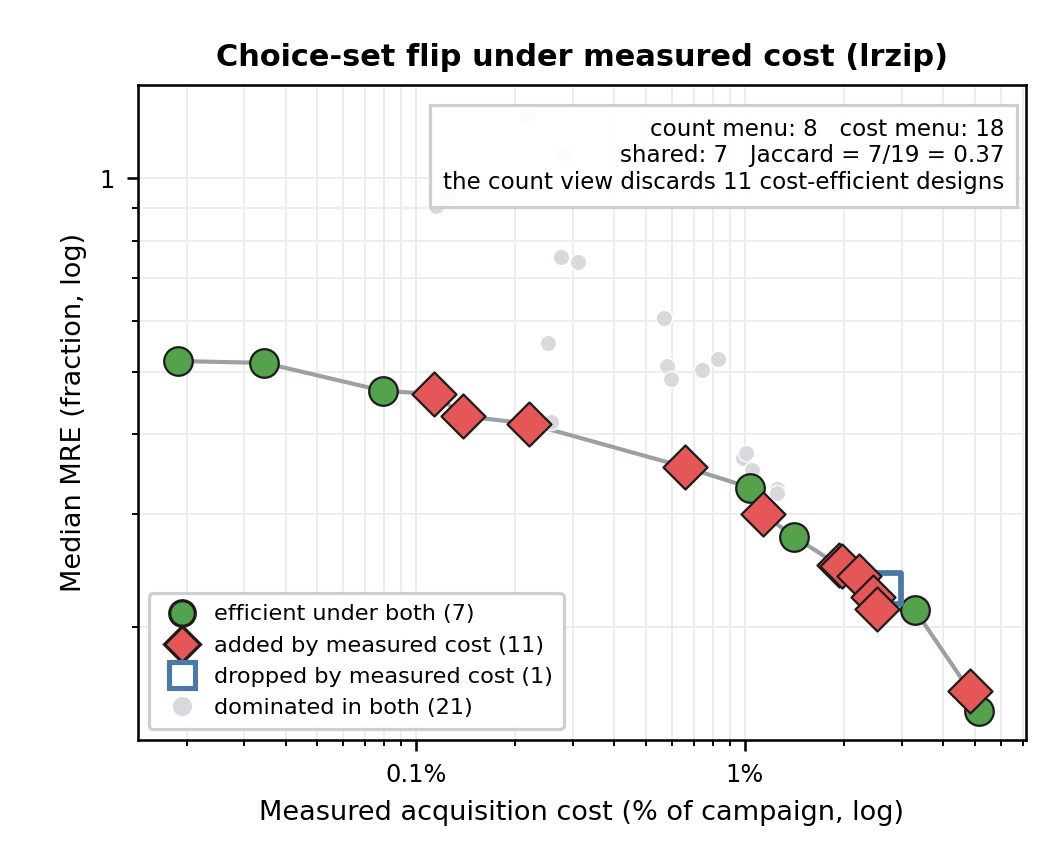
\includegraphics[width=0.9\columnwidth]{pic/results/choiceset_flip_lrzip.png}
\caption{The efficient choice set \emph{flips} under measured cost
(lrzip$\to$energy, the running example). Strategy--budget designs in the cost
decision space (lower-left better). Grey line is the measured-cost Pareto
frontier. The count and measured-cost menus ($8$ and $18$ designs) share only
$7$ (Jaccard $0.37$): measured cost adds $11$ (mostly cheap large-$n$
\texttt{pilotCost}) and drops $1$. The learner fits well ($0.15$ MRE), so this
is a real divergence, not an artifact.}
\label{fig:choiceset}
\end{figure}

The top-$1$ flip is the narrowest lens, and we report it as such. The single
best strategy--budget combination changes in $538/1{,}666$ context--weight
decisions ($32\%$). Most are near-ties in $J$, and the bootstrap-robust flips
($p_{\text{reproduce}}\ge0.95$) concentrate exactly where the KW and Pareto
lenses already move: where the target differs from the acquisition cost ($9$
robust x264 flips, all asymmetric) or cost is heavy-tailed (\StudyEnergy jump3r).
The flip corroborates the stronger lenses. It does not carry the claim alone. It
also underlines that the cost model is part of the experimental question: for
energy prediction the label is energy, but obtaining it requires running the
configuration, so execution time, not the target, is the natural acquisition
cost.

A changed verdict is not always ``the count winner was worse.'' Often it is more
accurate but costlier ($293/538$, $54\%$ of flips), so the question is whether
the accuracy gain is worth the budget. The remaining $188/538$ ($35\%$) are the
mirror case, cheaper but less accurate. ``Best at sample size $n$'' and ``best at
measured budget'' are simply different claims. The strict failures, the
$57/538$ ($11\%$) \emph{dominated} cases, are where no trade-off excuse exists:
a same-size or larger alternative is both cheaper and no less accurate, as in
\Cref{fig:running-example}. RQ2 therefore does not penalize accuracy. It asks
whether an accuracy advantage survives once the training-label resource is
charged.

\rqfinding{Answer to RQ2}{Measured cost changes sampling conclusions on their own
terms. At a fixed measured budget, the replication studies' own Kruskal--Wallis
test re-draws the set of statistically tied-best samplers in $38$--$55\%$ of
comparisons (all of them on Linux), and the change is most reproducible exactly
where the published verdicts live (every x264 change, $93\%$ on Linux, $75\%$ on
\StudyReplicationICSE). Sharper still, the source study's recommended sampler is
\emph{evicted} from the top group in $29$--$41\%$ of replication comparisons, and
the Pareto-efficient choice set robustly differs in $73$--$100\%$ of scenarios.
The single-winner flip agrees but is a fragile near-tie.}

\subsection{RQ3: Validity Conditions}
\label{subsec:results-rq3}

The count proxy is most defensible when per-configuration costs are tight, when
the target and acquisition resource are the same, and when the strategy does
not bias itself toward costly regions. It is most fragile when costs are
heavy-tailed, when target and cost differ, when workload or dataset changes the
cost distribution, or when the strategy explicitly seeks diversity or uncertain
regions.

\paragraph*{Why cost moves the verdict.} The mechanism is RQ1 propagating into
the sampler comparison. For a fixed strategy and size, MRE is a fixed number, so
re-pricing cost cannot change it directly. What changes is the cost-controlled
comparison: at an equal measured budget a cheap sampler affords a larger sample
(lower error) and an expensive one affords fewer (higher error), because the
size$\to$cost map is strategy-dependent (RQ1). Re-indexing operating points by
cost is thus a non-uniform permutation, not a rescaling, so the accuracy ranking
need not be preserved: \texttt{solverBased}, which selects expensive
configurations, repeatedly loses to \texttt{random} and \texttt{divDistBased} at
equal budget. The count proxy therefore fails precisely when per-configuration
costs are heterogeneous or the target differs from the paid resource.

Four recurring mechanisms explain why the proxy fails, in increasing severity:
(i)~a same-size choice can carry a large measured-cost gap (the count axis has
lost budget information, though the preferred sampler may be unchanged). (ii)~Two
choices can have similar MRE but very different cost (wasted budget without an
accuracy payoff). (iii)~A larger sample can be cheaper in measured time
(contradicting the monotone more-configurations-cost-more intuition).
(iv)~Classic same-budget configurable-system strategies can separate once
measured cost is charged: the case closest to prior sampling papers, showing
that even familiar fixed-nominal-budget comparisons can change under
heterogeneous cost. These are representative patterns, not exhaustive
evidence (\Cref{tab:rq-metrics} and the family paragraphs give that).

\begin{figure}[t]
\centering
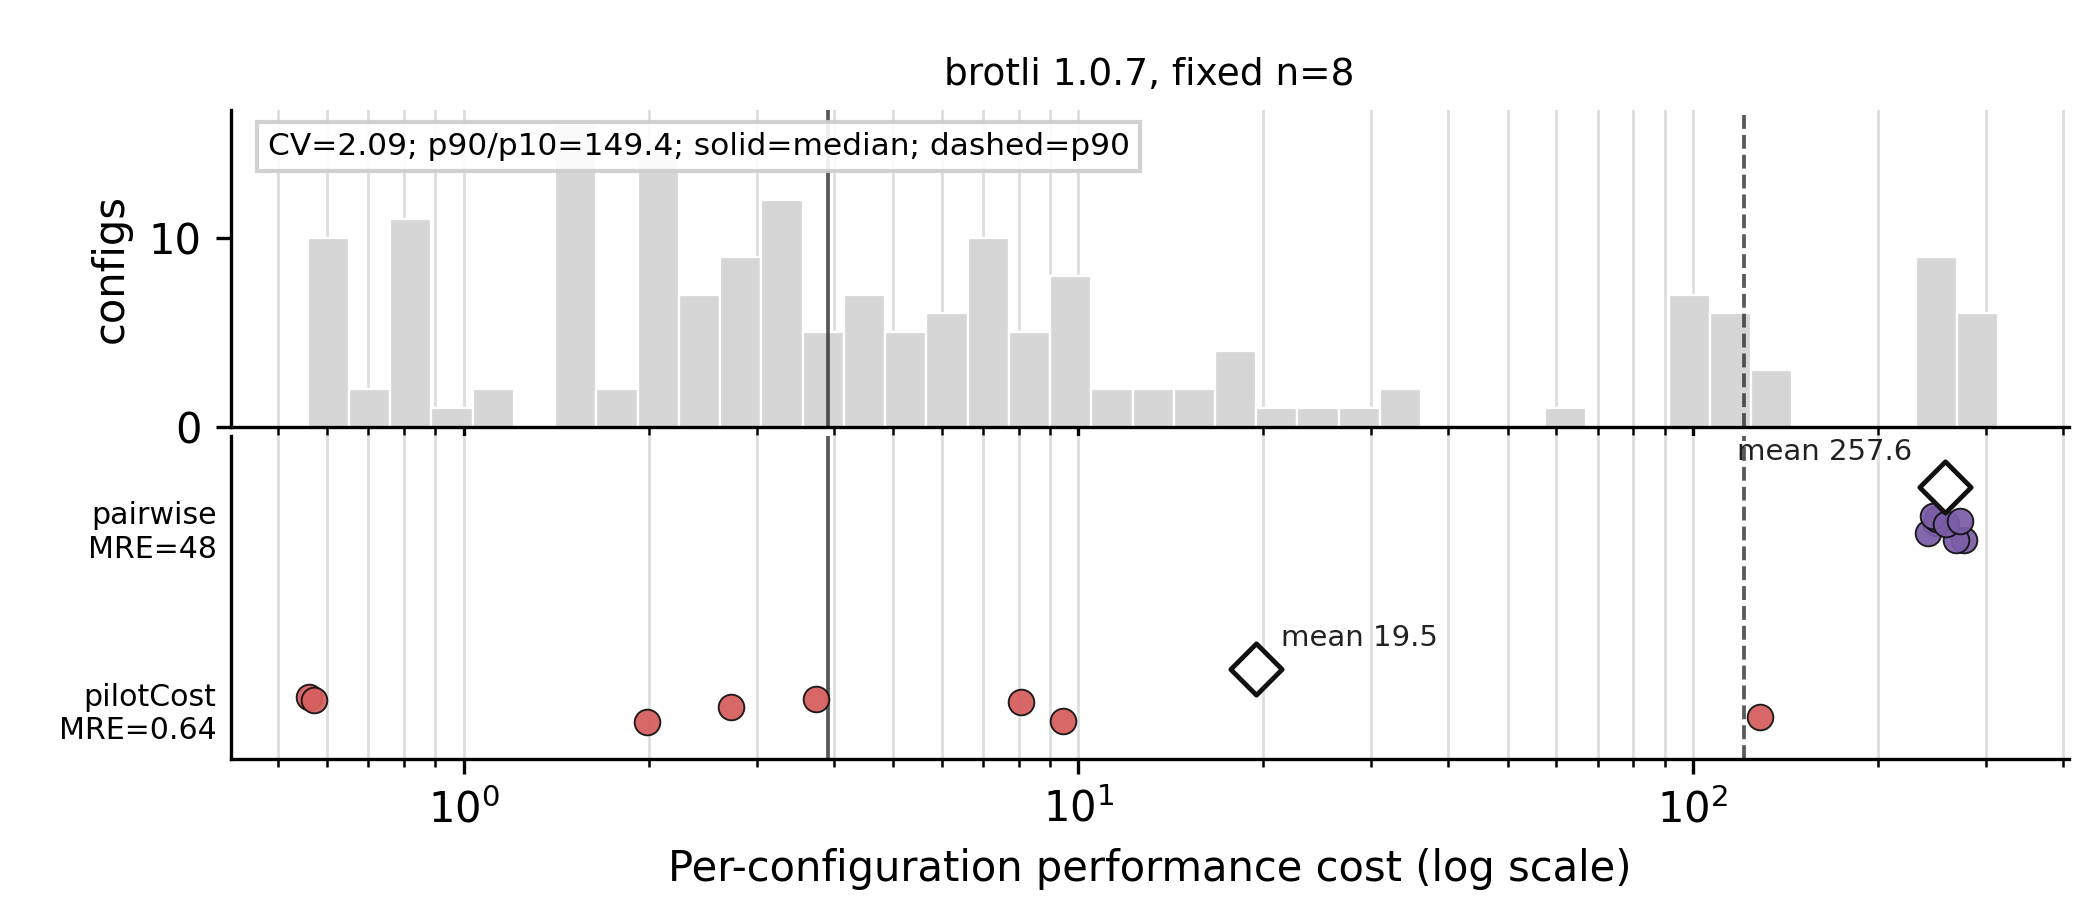
\includegraphics[width=\columnwidth]{pic/results/twins_brotli_fixed_n8_with_distribution.png}
\caption{Distribution-aware RQ3 example (brotli, fixed $n{=}8$). Top: the full
per-configuration performance-cost distribution. Bottom: where \texttt{pairwise}
and a representative \texttt{pilotCost} sample fall (circles = selected configs,
diamonds = sample mean, labels = energy MRE). \texttt{pairwise} selects the
expensive tail. \texttt{pilotCost} stays in the cheap bulk.}
\label{fig:brotli-distribution}
\end{figure}

\Cref{fig:brotli-distribution} opens one of these patterns by showing both the
strategy outcomes and the underlying cost distribution. All strategies use the
same $n=8$ count budget, yet pairwise selects eight configurations above the
full campaign's $p_{90}$ performance cost. Its mean selected cost is $257.6$,
it spends $31.2\%$ of the full measured budget, and its energy-prediction MRE is
$48.0$ (\ie predictions off by about $48\times$), because its expensive-tail
sample extrapolates poorly to the rest of the space. Pilot-cost is not an oracle for the cheapest configurations: in the
representative sample shown, its initial pilot includes one expensive point above
$p_{90}$ (and the pilot's own measurement cost is charged in $\TrainCost$, so the
strategy pays for the configurations it probes). Its cost-guided fill still places
the other seven selections in the low-to-mid-cost bulk, yielding mean selected
cost $19.5$, $2.36\%$ of the full measured budget, and MRE $0.64$ for that sample.

\paragraph*{Cross-RQ synthesis.}
The families fall into three practical regimes. In the \emph{validated-transfer}
regime, count-based conclusions survive the measured-cost check. LLVM, Polly,
Dune, HIPAcc, PostgreSQL, and x264 time/time are the main examples: costs are
tight enough, or the strategies are cost-unaware enough, that replacing count by
measured cost does not change the top recommendation. In the \emph{warning}
regime, the top recommendation mostly survives but the efficient choice set
changes. 7Z and BerkeleyDBC fit this pattern: a reader who only wants the single
winner may reach the same conclusion, but a reader comparing trade-offs would
miss measured-cost-efficient alternatives. In the \emph{changed-assessment}
regime, measured cost changes the recommendation itself. lrzip, the asymmetric
x264 time-cost/size-target scenario, heavy-tailed performance--energy systems,
many workload contexts, most \StudyLCBench datasets, and every Linux release
fall here. The scientific message is not that one sampler dominates in all
settings. It is that the validity of the count proxy is an empirical property of
the dataset, workload, cost dimension, and strategy panel. As a proof of concept
that these conditions are not merely narrative, a simple classifier over the RQ1
diagnostics ($p_{90}/p_{10}$, per-strategy $\Ratio$ spread, and target--cost
asymmetry) identifies where measured cost \emph{materially} changes the
recommended sampler. Across the $167$ contexts (each a system, input, workload,
dataset, or release), the ones it ranks high-risk change in $85\%$ of cases versus
$32\%$ for the rest (five-fold cross-validated, AUC $\approx0.78$, driven mainly by
cost spread)~\cite{artifact}.

\rqfinding{Answer to RQ3}{Sample size is safest as a cost proxy when
per-configuration costs are tight, the target and bottleneck resource coincide,
and strategies are cost-unaware. It is unsafe when costs are heavy-tailed,
target and acquisition cost differ, workload or dataset changes the cost
distribution, or the strategy deliberately searches unusual, diverse, or
uncertain regions.}

\section{Discussion and Threats to Validity}
\label{sec:discussion}

\paragraph*{Implications for the state of the art.}
Most configurable-system sampling work pursues \emph{cost-effectiveness}, a useful
accuracy at an affordable measurement effort, rather than the lowest possible
error. Cost-efficient, distance-based, $t$-wise, and active-learning strategies are
justified by spending less for comparable accuracy, yet that effort is almost
always reported as a sample count, and RQ1 shows the count is not the budget that
is spent. A cost-effectiveness claim stated in counts is therefore unverified, and
it can be wrong: in RQ2, at a fixed measured budget the set of statistically best
samplers changes in $38$--$55\%$ of the replicated comparisons and on every Linux
release, and the sampler the literature credits is often not the cost-effective
one. Solver-based $t$-wise sampling, recommended on x264, selects expensive
configurations and loses once time is charged, while \texttt{random}, treated as a
weak baseline, is the most over-credited by count. This is not a footnote: part of
the state of the art recommends samplers that are not as cost-effective as claimed,
so a cost or efficiency claim should henceforth be established against measured
cost rather than assumed from $n$.

\paragraph*{Navigating the cost--accuracy trade-off.}
Once cost is measured, the choice is a front, not a point. Strategy--budget
combinations form a Pareto set in the accuracy--cost plane, and the RQ2
measured-cost front differs from the count-based one in $73$--$100\%$ of scenarios. The practical
decision is to pick the operating point that reaches the accuracy a study needs at
the least measured cost, rather than fixing $n$ and reporting whatever accuracy
follows. A few choices strictly dominate, being cheaper \emph{and} more accurate,
and are unambiguous wins. The rest are genuine trade-offs, and the value of
measuring cost is that the practitioner can see and navigate them instead of
having them collapsed behind a common count.

\paragraph*{Guidance for researchers and practitioners.}
The reporting change is lightweight. State the cost dimension, report both sample
size $n$ and measured cost $\TrainCost$, and show whether the two budgets agree
through the RQ1 diagnostics, cost spread and per-strategy $\Ratio$, since a global
average hides a consistently cheap or expensive strategy. If costs are homogeneous
and ratios stay near $1$, count is a defensible proxy, the validated regime of
RQ3. Otherwise, recompute the
accuracy--cost ranking and Pareto front under measured cost and label which
conclusions are count-based and which are measured-cost based. The opportunity is
concrete and now quantified: count-based sampling leaves measurable
cost-effectiveness on the table, and \texttt{pilotCost} already recovers part of
it, reaching better accuracy at equal measured budget on several systems. It can
fail where cheap regions are uninformative, but the gap we measure, largest under
heavy-tailed costs, is a clear motivation and a sizable target for the cost-aware
samplers that future work can design.

\paragraph*{Sampling strategy choice is subject-specific (panel validity).}
The choice of sampling strategies could itself drive the result. One concrete
hypothesis is that the cost-aware \texttt{pilotCost} sampler we add explains most
of the changes. We test this hypothesis with an experiment: we remove
\texttt{pilotCost} and the cost-aware bounds and re-run the comparison with only
the cost-unaware \texttt{random} and \texttt{balanced} samplers. The measured-cost
top group still changes in $59\%$ of \StudyEnergy, $52\%$ of \StudyWorkload, and
$32\%$ of \StudyLCBench\ comparisons (versus $50/46/42\%$ with the full set), the
count-recommended sampler is evicted in up to $22\%$, and Pareto fronts still
differ in $62$--$71\%$ of scenarios. The effect is thus a property of the cost
axis, not of the sampler we add, and the statistical verdicts are robust to
dropping it. Along the way the experiment teaches something more general: even
among cost-unaware samplers the cost-effective choice is subject- and
budget-specific, so practitioners should choose per subject rather than assume a
universal best. Consistently, the change also holds on the two replications and
\StudyLinux, which contain no cost-aware sampler and reuse the published
\StudyReplicationICSE\ and \StudyReplicationICPE\ strategy sets unchanged.

\paragraph*{Construct validity (what ``cost'' includes).}
We charge the measured cost of \emph{acquiring} the selected training
configurations, not the cost of \emph{selecting} them: constraint solving,
pairwise-distance computation, or active-learning retraining. This scope is
deliberate and conservative: prior sampling studies measure effort as sample
\emph{size} and thus ignore selection cost as well, so our cost axis is already a
strict improvement on the count baseline we compare against, and because most
strategies select a sample once and for all, any selection cost is amortized over
the campaign and small beside measurement.

\paragraph*{Internal validity (learners, seeds, grid).}
Prediction error, and thus which sampler wins RQ2 and RQ3, can depend on the
learner and on sampling noise (RQ1 does not, as it precedes any model fit). To
mitigate this we keep the replication studies' original ridge learner and re-run
the entire decision analysis under CART and the scikit-learn random forest
\cite{sklearn_api}, with gradient boosting on the high-dimensional Linux space,
which agrees with the random forest.
The strong learners cut error sharply (median MRE on \StudyReplicationICSE\
$0.26{\to}0.07$) yet do not restore the count proxy: count-versus-measured
top-choice agreement stays at $0.43$--$0.81$ and measured-cost Pareto fronts still
differ (Jaccard $0.30$--$0.57$). We average over repeated seeds (about $100$ runs
per cell for the replication archives and $30$ for the generated families) and
bootstrap every reported proportion ($B{=}1000$). Because sample sizes are
discrete, we judge decisions by Pareto changes across the size grid, not at a
single budget point.



\paragraph*{External validity.}
The systems span compilers, encoders, databases, archivers, energy, workloads,
machine-learning runtime, and Linux releases, all real configurable software
measured in prior studies rather than synthetic, though still a finite, curated
set, and we run many per-scope tests. We therefore report the families separately and rest
the claims on patterns that repeat across them rather than on any single test. A
system that recurs in two families is not a redundant replicate: it is measured on
a different non-functional property and context (x264, for instance, contributes
encoding time and output size over $17$ videos in \StudyReplicationICPE\ but
energy in \StudyEnergy), so agreement across families is evidence over genuinely
different measurement settings, not the same one repeated. Per-scope statistics,
$p$-values, and effect sizes are in the anonymized artifact~\cite{artifact}.

\section{Conclusion}
\label{sec:conclusion}

Sampling cost matters. For configurable-system performance prediction, the
number of measured configurations is a useful summary but not a resource budget
unless checked against measured cost: across the systems we studied,
$n$ almost always orders measured cost, yet it can misstate the budget, hide
strategy-specific bias, and change which strategy or strategy--budget combination
is recommended.

We quantify this with the replication studies' own test. Rerunning their
Kruskal--Wallis best-sampler comparison at a fixed measured budget rather than a
fixed sample size changes the set of statistically tied-best samplers in
$38$--$55\%$ of comparisons across the five non-Linux families (and $100\%$ on
\StudyLinux), most reproducibly on the replications and Linux. The measured-cost
Pareto-efficient choice set, the stabler decision-level evidence, robustly differs
in $73$--$100\%$ of scenarios. This is a validity warning, not a systematic rejection: count-based
effort is defensible for homogeneous systems and cost-unaware samplers (we identify
several), and unsafe under heavy-tailed costs, target--cost asymmetry,
workload-sensitive distributions, dataset shifts, and diversity or
active-learning strategies that drift toward costly regions.
%: conditions common,
%measurable, and severe enough to change winners and fronts.

The stronger lesson is effectiveness: a sampler can look effective by being
accurate at a small \emph{count} budget while silently spending a large
\emph{measured} one, or look unattractive while actually costing less. Sample
count alone therefore cannot establish which strategy is cost-effective. It also
reveals an opportunity: samplers that deliberately target cheap-to-measure
configurations, and measuring cost is the first step toward designing them.

\smallskip\noindent\textbf{Open science.} Data, configurations, seeds, costs, and
reproduction scripts are in the anonymized artifact~\cite{artifact}.

\smallskip\noindent\textbf{Use of AI Assistants.} Claude Code was carefully used to assist with code
implementation and paraphrasing during paper writing. All scientific content,
experimental design, analysis, and claims are entirely the authors' own.


%\section*{Acknowledgments}
%Anonymized for review.

\newpage
\bibliographystyle{IEEEtran}
\bibliography{MYfull,ml,macher,jhipster}

\end{document}
